\documentclass{article}
\usepackage{listings} % 引入代码展示宏包
\usepackage{xcolor}
\lstset{
  backgroundcolor=\color{gray!10},      % 背景色:浅灰色
  basicstyle=\ttfamily\footnotesize,    % 基本样式:等宽字体,小号字体大小
  breakatwhitespace=false,              % 是否只在空白处自动断行
  breaklines=true,                      % 自动断行
  captionpos=b,                         % 标题位置:底部
  commentstyle=\color{green},           % 注释样式:绿色
  deletekeywords={...},                 % 删除的关键字
  escapeinside={\%*}{*)},               % LaTeX代码内嵌的转义符
  extendedchars=true,                   % 启用非ASCII字符
  frame=single,                         % 边框样式:单线边框
  keepspaces=true,                      % 保持空格,有助于保持代码的缩进
  keywordstyle=\color{blue},            % 关键字样式:蓝色
  language=bash,                        % 代码语言:Bash(Linux命令行)
  morekeywords={*,...},                 % 添加的关键字
  numbers=left,                         % 行号位置:左侧
  numbersep=5pt,                        % 行号与代码的距离
  numberstyle=\tiny\color{gray},        % 行号样式:小号字体,灰色
  rulecolor=\color{black},              % 边框颜色:黑色
  showspaces=false,                     % 不显示空格标记
  showstringspaces=false,               % 字符串中不显示空格标记
  showtabs=false,                       % 不显示制表符标记
  stepnumber=1,                         % 行号步进:每行显示
  stringstyle=\color{purple},           % 字符串样式:紫色
  tabsize=2,                            % 制表符大小
  title=\lstname                        % 显示文件名
}
\usepackage{multirow}
\usepackage{pgfplots}
\usepackage{ifthen}
\usepackage[UTF8]{ctex}
\usepackage[left=3.18cm,right=3.18cm,top=2.54cm,bottom=2.54cm]{geometry}
\geometry{a4paper}
\usepackage{tikz}
\usetikzlibrary{chains}
\newcommand{\diff}{\mathop{}\!\mathrm{d}}
\usepackage{appendix} 
\usepackage{diagbox}
\usepackage{pdfpages}
\usepackage{subcaption}
\usepackage{algorithm}
\usepackage{algpseudocode}
\renewcommand{\algorithmicrequire}{\textbf{Input:}}  
\renewcommand{\algorithmicensure}{\textbf{Output:}}  
\usepackage{amsmath}
\usepackage{amsthm}
\DeclareMathOperator{\sigm}{sigm}
\usepackage{graphicx} 
\usepackage{float}
\renewcommand{\vec}[1]{\boldsymbol{#1}}
\usepackage{amssymb}
\usepackage{booktabs} 
\usepackage{hyperref}
\usepackage{titlesec}
\usepackage{caption}
\captionsetup{font={small,bf}} 
\bibliographystyle{plain}
\newtheorem{definition}{定义}
\newtheorem{lemma}{引理}
\newtheorem{theorem}{定理}
\DeclareMathOperator{\Ima}{Im}
\DeclareMathOperator{\Rank}{rank}
\begin{document} \pingfang
\begin{center}
    \textbf{\huge 数据库(2)实验1:云服务器部署Mysql}
\end{center}
\begin{center}
    \textbf{\large \textbf{学号:21121178 \quad 姓名:王士博 \quad 指导教师:刘洋}}
\end{center}
\hrulefill
\section{实验要求}
\begin{itemize}
  \item 建立两台云服务器之间的不安防(Server 和 Client),并实现两个实例之间的SSH免密登录。
  \item 两个实例上安装MySQL,在Server上创建数据库和用户,在Client上远程连接Server和Client。
\end{itemize}
\section{实验内容}
\subsection{构建两个云服务器实例}
实验前提是已经购买了两个2GB的实例,操作系统为Ubuntu 20.04,设置两个实例的名称分别为Server和Client,共开放配置安全组,添加规则,添加MySQL(3306)。
\subsection{前置软件安装}
\begin{lstlisting}[language=bash]
sudo apt-get update
sudo apt-get install vim
sudo apt-get install openssh-server
sudo apt-get install mysql-server
\end{lstlisting}
\subsection{SSH免密登录}

在client端创建公钥和私钥。然后将id\_rsa.pub文件中的内容写入到authorized\_keys文件,就可以在client端免密码登录SSH登录loaclhost,
然后再通过scp(Secure Copy Protocol)复制到server的/home/ubuntu/.ssh目录下,即可两机本身和相互之间都可以
实现无密码ssh登陆。
\begin{figure}[ht]
    \centering
    \begin{subfigure}[b]{0.4\textwidth} 
        \centering
        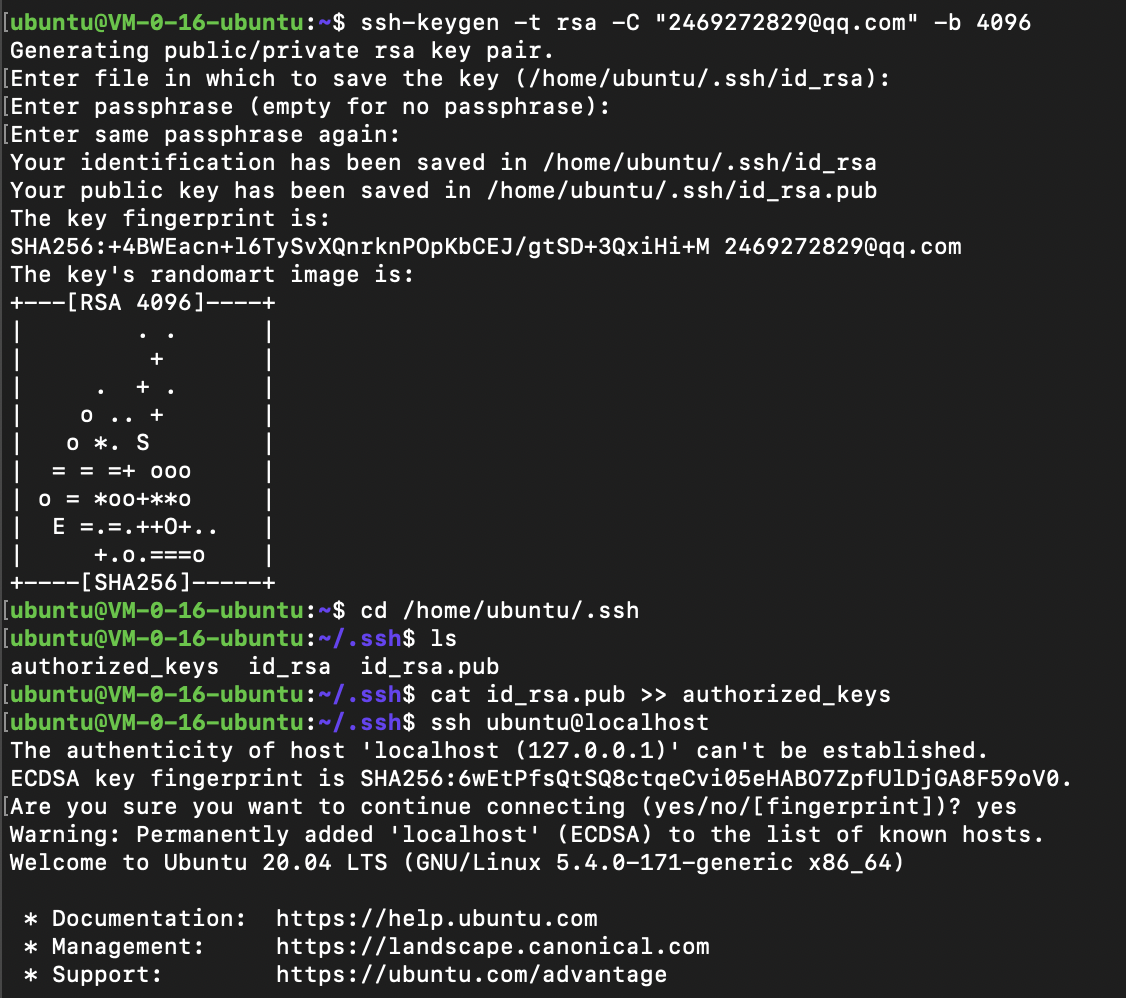
\includegraphics[width=\textwidth]{client_login_ssh.png} 
        \caption{在Client端创建公钥和私钥并且实现无密码ssh登录}
    \end{subfigure}
    ~
    \begin{subfigure}[b]{0.4\textwidth}
        \centering
        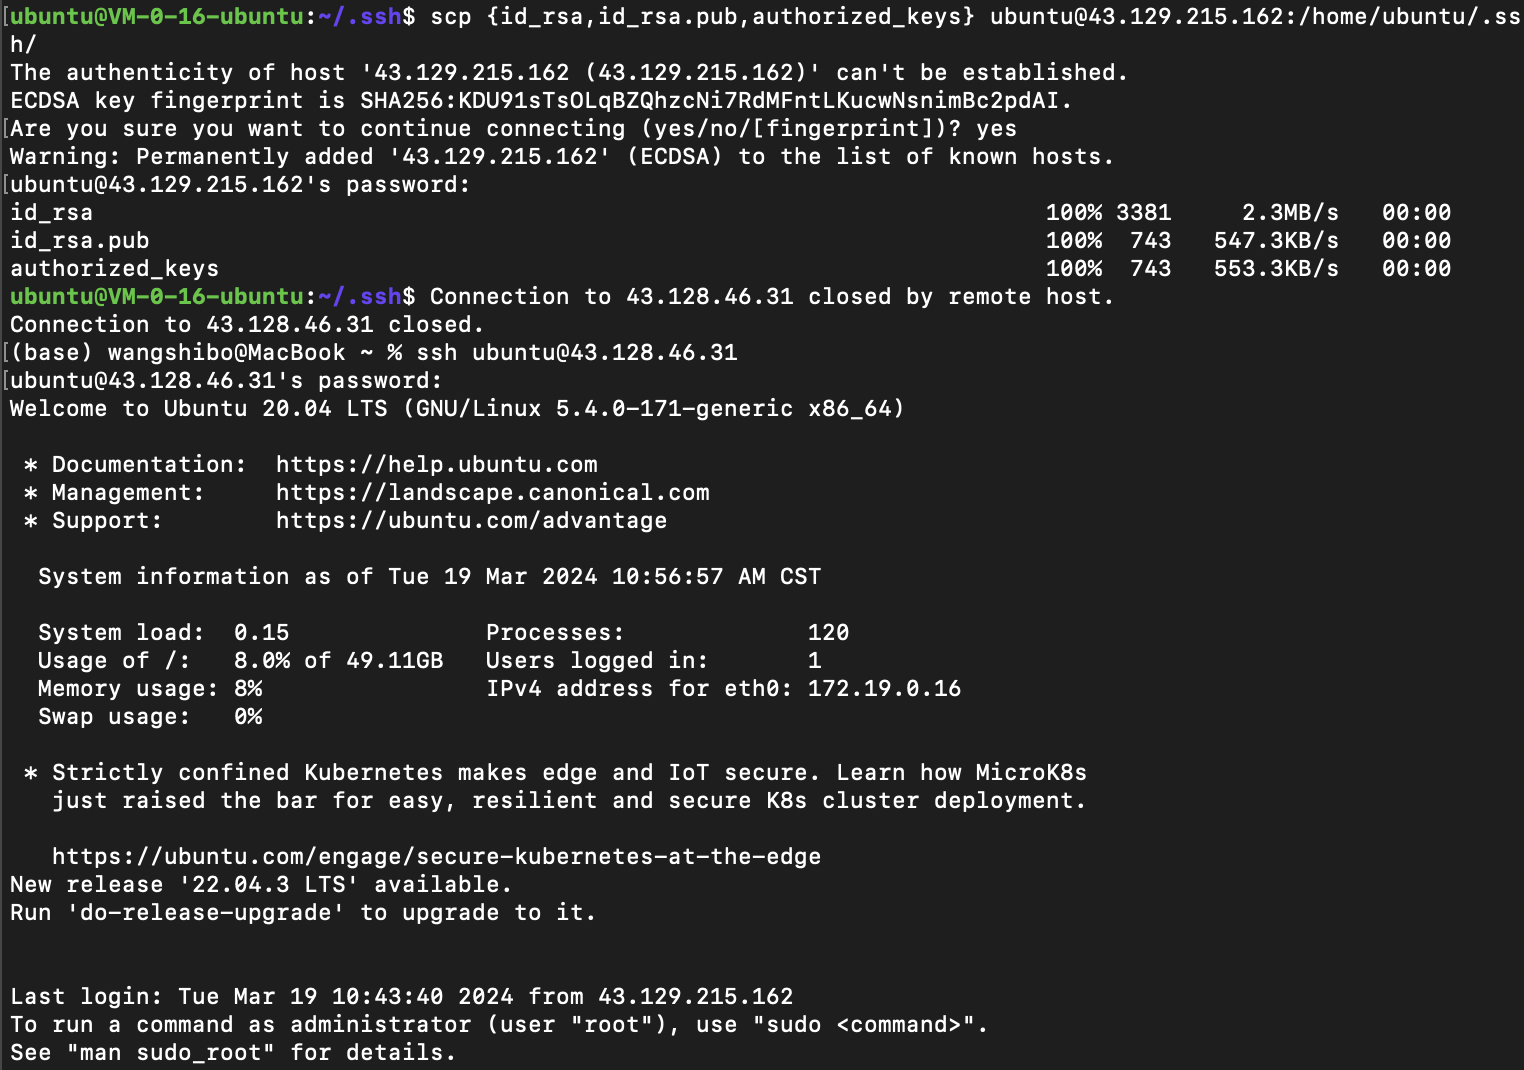
\includegraphics[width=\textwidth]{scp_ssh_without_pwd.png}
        \caption{通过scp复制到Server端实现无密码ssh登录}
    \end{subfigure}
\end{figure}

\begin{lstlisting}[language=bash]
ssh-keygen -t rsa -C "LIXTT"
cd .ssh
cat id_rsa.pub >> authorized_keys
cat authorized_keys
\end{lstlisting}

\subsection{创建数据库和用户}

使用apt-get工具安装mysql-server之后,在server端,用vim工具更改配置文件,将mysql.conf.d文件夹中的mysqld.cnf中的bind-address从"127.0.0.1"修改为"0.0.0.0"
(或者直接注释掉这一行),然后重启Mysql服务让配置文件生效。按照下面的命令创建测试数据库和用户
然后就可以使用client端实现-h来制定host登陆server的数据库了。
\begin{lstlisting}[language=bash]
sudo mysql -u root -p
mysql>CREATE DATABASE Test;
mysql>CREATE USER 'client'@'172.19.0.16' IDENTIFIED BY '114514';
mysql>GRANT ALL ON *.* TO 'client'@'172.19.0.16';
mysql>FLUSH PRIVILEGES;
\end{lstlisting}
\begin{figure}
    \centering
    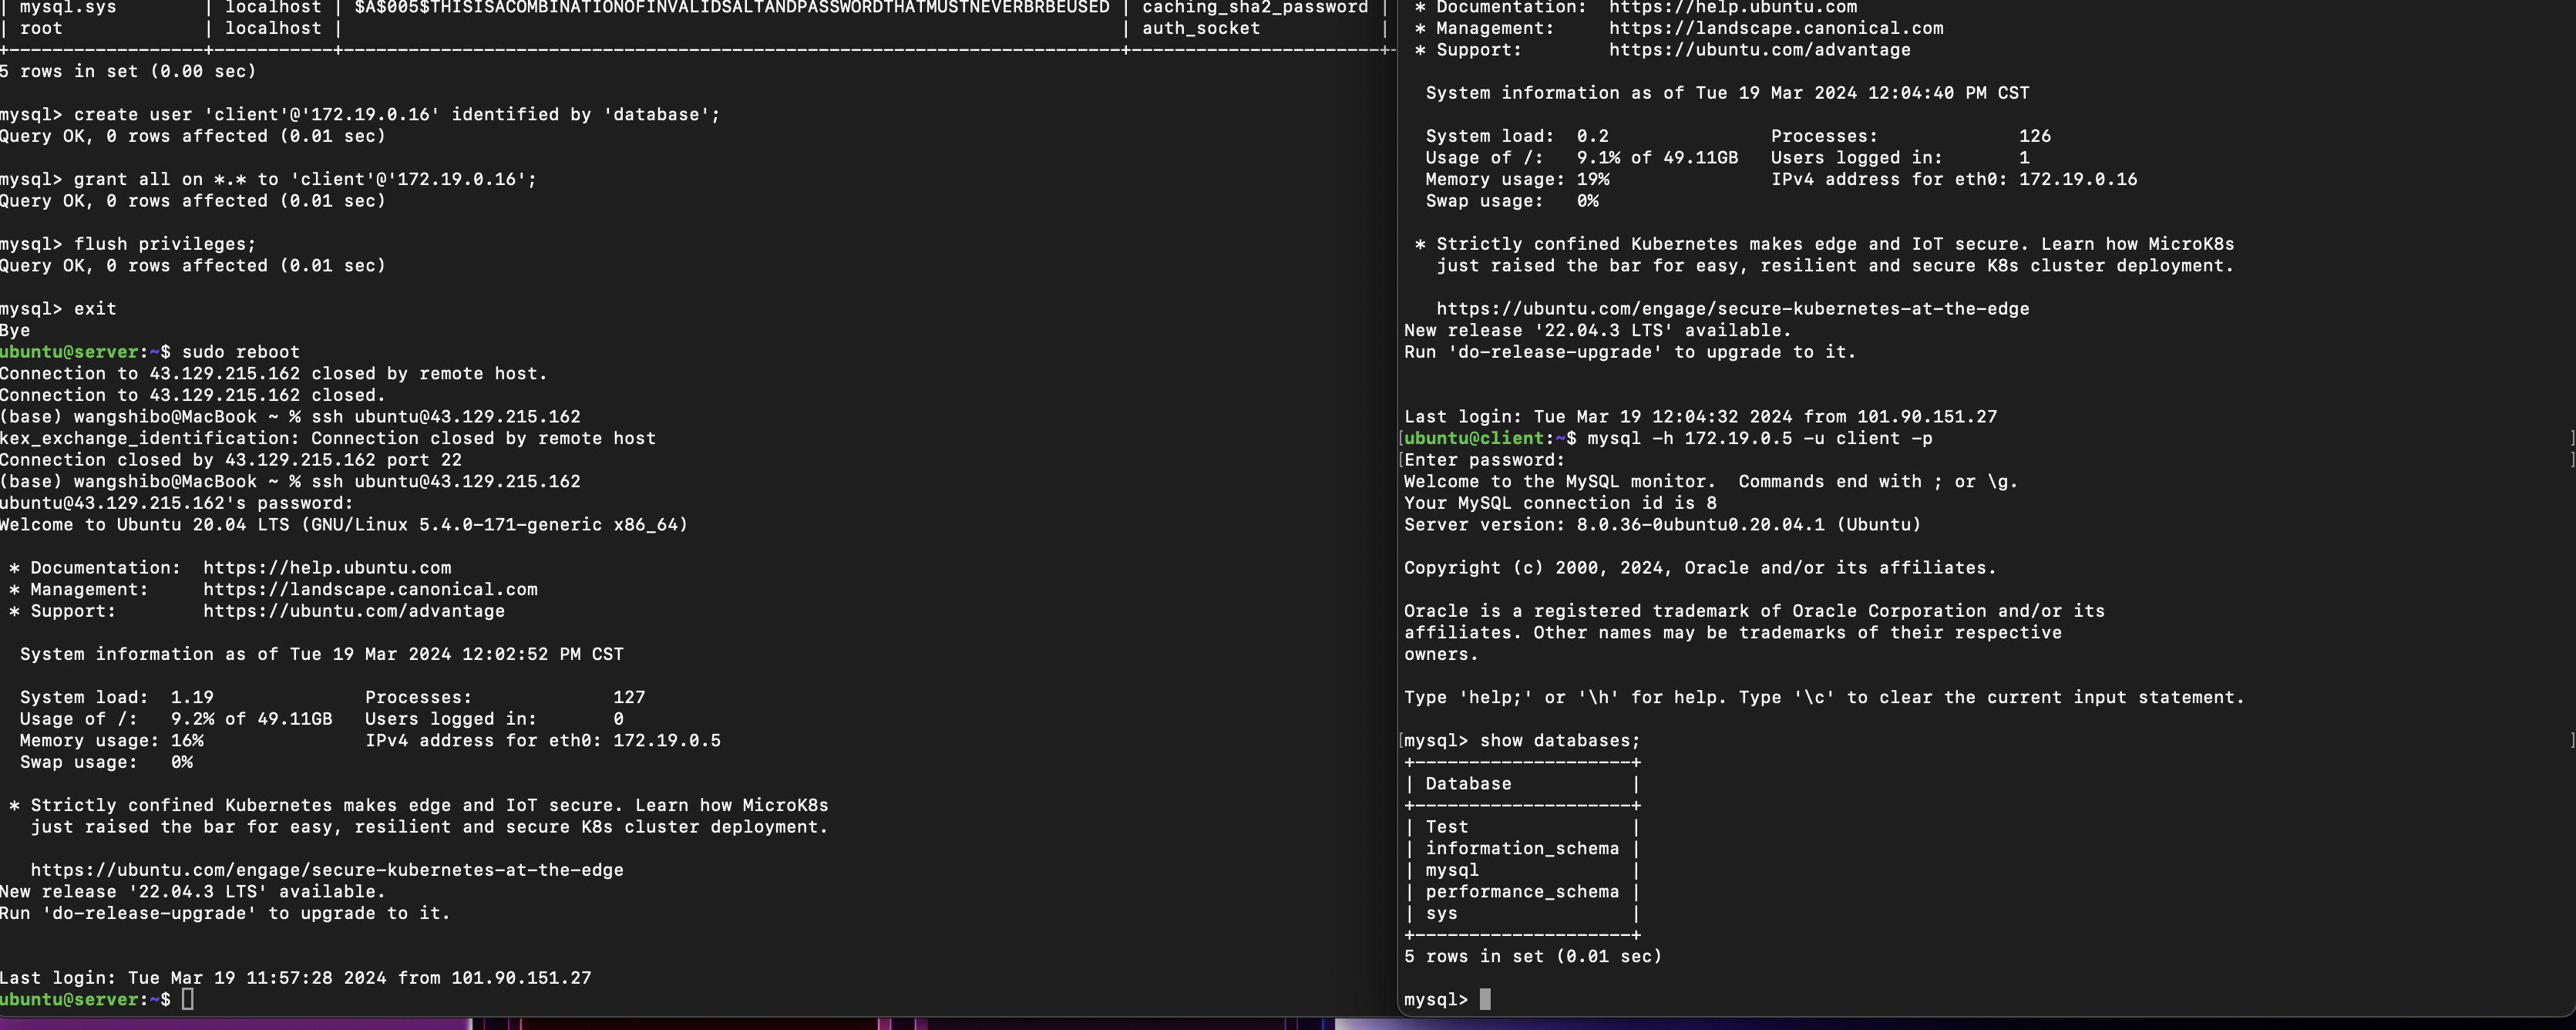
\includegraphics[width=1.0\textwidth]{deploy_mysql.png}
    \caption{部在server部署数据库并且在client上远程登录数据库}
\end{figure}
\end{document}
